%!TEX root = main.tex
\section{Introduction}
\subsection{Context}

\begin{figure*}[!t]
	\centering
	\begin{minipage}{0.9\linewidth}
		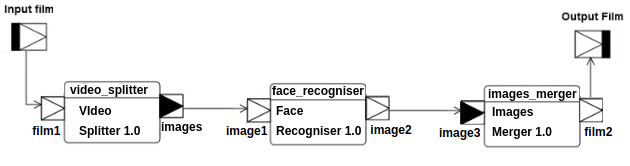
\includegraphics[width=1.0\textwidth]{face_recogniser_app}
	\end{minipage}
	\caption{\textit{Face Recogniser} scheme. Application written in the CAL language.}
	\label{fig:face_recogniser_app}
\end{figure*}

The research described in the article focuses on providing the tool for estimating the run-time of a single CAL module (data processing program or algorithm). Computation Application Language (CAL) is designed to write large-scale applications due to perform big data processing. Each CAL program consists of separately executed modules in sequence (with parallelization possibility) on virtual machines and sending the results further to the next module of the application. CAL language is a part of the system developed under the Baltic LSC\cite{baltic_lsc_website} project.

During the data processing within the application run, each module is executed with some input data. It could be a different kind of data e.g. data frame or set of images. The execution of a module is invoked on a virtual machine with limited resources (RAM, mCPUs, GPUs). The properties of input data and the execution environment resources will be used by models to estimate the overall application execution time and price on a specific cluster.

Baltic Large Scale Computing (BalticLSC\cite{baltic_lsc}) project is using CAL language to perform data processing tasks. Each task is an execution of a CAL application. CAL applications can use each module of the system in a reusable way. We can say that a single module is one block (commonly as a docker image) and an application is a schema of executing a sequence of blocks. Figure~\ref{fig:face_recogniser_app} shows the example application that consists of a few modules to perform face recognition on the input video data. Some sets of modules within a CAL application can be executed in parallel. Some modules can also be run as multiple instances of themselves to make data processing faster.

The demand for large-scale computation is tremendous and it is growing all the time. Mostly because of the high computational requirements of machine learning models and other tasks related to the Big Data thinks such as the Internet of Things~\cite{iot}. To execute the computations, it takes a lot of hardware resources. Moreover, it is really frequent that data processing programs have common parts that could be shared between them to make the whole process of the program's engineering more granulated and universal. Focused on just one-step of processing, an engineer could provide a well optimized module that could be shared in many programs. The BalticLSC project's research focuses on providing the complete system, handling mentioned challenges of large-scale computing.

\subsection{Issue}

The worst-case complexity of an algorithm is the greatest number of operations needed to solve the problem over input data of a given size. The analysis of algorithmic complexity emerged as a scientific subject during the 1960s and has been quickly established as one of the most active fields of study\cite{complexity}. The most common way to describe an algorithm complexity is the \textit{big O} notation (collectively called Bachmann–Landau notation or asymptotic notation) which is the universal formula that describes how the run-time of an algorithm grows as the input data size grows. 

In our work, we study the formula (more precise and complex one in comparison to the \textit{big O} notation) that takes mixed sets of input data and run-time environment properties as arguments. Moreover, the models we introduce in further parts will provide the estimation of the data processing program run-time and not only the complexity formula as the \textit{big O} notation does.

\subsection{Related work}

Since run-time estimation is a long-known issue, it is commonly studied from different perspectives and various approaches. There are many articles that, to some extent, coincides with the research carried out in this article. An overview of the problem with the list of possible, known solutions is described in the \textit{estimation of the execution time in real-time systems}\cite{wcet}. The authors focus on the \textit{WCET} concept. This project aims not to estimate execution time as a deadline that could not be exceeded. In our work, we try to estimate the average-case execution time (\textit{ACET}), which has a loser requirement for the final upper bound of the run-time than the \textit{WCET}.

A similar approach to the run-time estimation have been introduce in the \textit{Execution Time Analysis for Embedded Real-Time Systems}\cite{time-analysis} - as is said in the section 5. of the article, a static timing  analysis tool works by statically analysing the properties of the program (embedded to a specific structure like vector or graph) that affect its timing behavior. On the other hand, our approach is to statically analyze the properties of input data and the run-time environment resources. It allows to focus more on a single program and receive more accurate results. However, we have to provide a sufficient amount of input data for each module what is challenging. The fact that analysing programs run in BalticLSC system and they are reusable we assume that each module will be repeatedly triggered and it allows to carry enough data.  

In section 3.6 of the \textit{Using online worst-case execution time analysis and alternative tasks in real-time systems}\cite{images-processing-time} we can find a similar approach to carry out the regression using input data feature (section 3.6). The authors use an amount of image pixels as the only feature to estimate the execution time of a few different image processing algorithms. This is only a part of the whole approach for the worst-case execution time analysis described in the article, but it is the most related one to our work. It is worth noticing that there could be some specific input data properties for each algorithm that substantially impact the run-time. Models that we studied have general, strictly limited features, the same ones for each module, but one can extend it with some specific properties of a module.

To get a more precise run-time estimation results, one can study the program with similar input data. In the article \textit{A Prediction Model for Measurement-Based Timing Analysis}\cite{ga} the authors made an experiment by generating random lists of data with the same properties and then train the artificial neural network to predict the \textit{WCET}. They used \textit{Gem5} to simulate the run-time environment. We have used the docker as an execution environment which allows receiving more real data with a natural noise introduce to the response variable (execution time). The authors develop their work in the next article\cite{surogate} using the concept of surrogate models as a solution to the problem of generating training data. Such generating can increase overheads of the execution time estimation for processing algorithms with heavy input data. It is worth considering as an extension of our approach to generating some input data when the module is new and does not have any executions yet.

If we know that there will be not enough execution of each program within some system, we can create a single model for a whole system. The authors within the article \textit{Nonlinear approach for estimating WCET during programming phase}\cite{program-features} estimate a \textit{WCET} by extracting the program features from the object code. It starts when the source code of a program is successfully compiled into object code. Then, the extracted features were used for subsequent sample optimization and \textit{WCET} estimate. The authors use the SVR algorithm with RBF kelner as we did likewise. Having a set of features for each program, we can unify a model to a single instance and provide the features as a part of input data for the model. Another clue to the not enough amount of input data for a model is described in the article \textit{A solution to minimum sample size for regressions}\cite{small-n}. The authors explore the problem of a small amount of training data which also affects the result of our article. Testing data generation and simple algorithms for the run-time estimation are used to reduce the impact of a small n problem on the final results of our work.

\subsection{Contribution}

Despite the widely studied subject of estimating a program execution time, there is always a place to improve. Our work, presented in the article, contributes to the current knowledge of run-time estimation. We offer another perspective of solving the problem and one can find some valuable aspects of our work.

Most importantly, we used simple machine learning algorithms (\textit{SVR} and \textit{KNN}, more about the algorithms and how they fit the problem in the further sections) to estimate a program run-time. Creating a separate model for each module (program) instead of embedding the program structure to a vector of features or control flow graphs (CFGs) allows being more focused on each module separately. As input data features for our models, we determined the basic properties of a program’s input data together with the properties of the run-time environment of an execution. 


